\documentclass[a4paper,11pt,twoside]{report}

% Title and authors
\newcommand{\theTitle}{Statistical analysis of forestry data}
\newcommand{\theShortTitle}{Analysis of forest Inventory data} 
\newcommand{\theAuthor}{Brian Crowley}
\newcommand{\theShortAuthor}{15167763}

% Bibliography style
%\usepackage{cite}
%\usepackage{natbib}
% Useful for sorting and compressing citations
%\bibliographystyle{abbrv}

%\usepackage[
backend=biber,
style=alphabetic,
sorting=ynt
]{biblatex}
 %\usepackage{csquotes}

%\addbibresource{FYP.bib}

% Page style
\usepackage{enumitem}
\usepackage[a4paper,top=2.5cm,bottom=2.5cm,outer=2.5cm,inner=2.5cm,includeheadfoot]{geometry}
\usepackage[utf8]{inputenc}
\usepackage{tabu}
\usepackage{fancyhdr}
\pagestyle{fancy}
\headheight=18pt
\footskip=24pt
\fancyhf{}
\renewcommand{\chaptermark}[1]{\markboth{}{#1}} 
\fancyhead[RO,LE]{\bfseries \theShortTitle}
\fancyhead[LO,RE]{\bfseries \rightmark}
\fancyfoot[C]{\thepage}

% Spacing
\usepackage{setspace}
\onehalfspacing
\usepackage{parskip}

% AMS Packages for maths typesetting
\usepackage{amsmath}
\usepackage{amsfonts}
\usepackage{amssymb}
\usepackage{listings}


% Importing graphics and defining graphics path
% NOTE: This means you can put graphics in a Figures subfolder and LaTeX will find them.
\usepackage{graphicx}
\graphicspath{{./}{./Figures/}}

% TikZ packages and useful libraries
% Useful for drawing your own figures and plots in LaTeX (see TikZ/PGF and PGFplots manuals online for details)
\usepackage{tikz}
\usepackage{pgfplots}
\pgfplotsset{compat=1.15}
\usetikzlibrary{calc}
\usetikzlibrary{plotmarks}
\usetikzlibrary{patterns}
\usetikzlibrary{shapes}
\usetikzlibrary{positioning}
\usepackage{subcaption}

% Languages
\usepackage[english]{babel}

% Miscellaneous packages
\usepackage{hhline}               % Better lines in tables

%%%%%%%% USER DEFINED COMMANDS (you can make your own of these, these are the basics that I frequently use)
% Note that it is bad practice to introduce user defined commands to shorten things like \begin{environment-name} or \end{environment-name}.

% Calculus
\newcommand{\dee}{\mathrm{d}}
\newcommand{\Dee}{\mathrm{D}}
\newcommand{\diff}[2]{\frac{\mathrm{d} #1}{\mathrm{d} #2}}
\newcommand{\ddiff}[2]{\frac{\mathrm{d}^2 #1}{\mathrm{d} #2^2}}
\newcommand{\pdiff}[2]{\frac{\partial #1}{\partial #2}}
\newcommand{\pddiff}[2]{\frac{\partial^2 #1}{\partial #2^2}}
\newcommand{\mdiff}[2]{\frac{\mathrm{D} #1}{\mathrm{D} #2}}

% In text
\newcommand{\ie}{\emph{i.e.}\ }
\newcommand{\eg}{\emph{e.g.}\ }
\newcommand{\etc}{\emph{etc.}}
\newcommand{\etal}{\emph{et al.}\ }
\newcommand{\etalp}{\emph{et al.}}

% Useful functions
\newcommand{\floor}[1]{\left\lfloor #1 \right\rfloor}
\newcommand{\ceil}[1]{\left\lceil #1 \right\rceil}

% Operator names
\newcommand{\tr}{\operatorname{tr}}
\newcommand{\cof}{\operatorname{cof}}
\newcommand{\sym}{\operatorname{sym}}
\newcommand{\skw}{\operatorname{skw}}
\newcommand{\erf}{\operatorname{erf}}
\newcommand{\diag}{\operatorname{diag}}
\newcommand{\sech}{\operatorname{sech}}
\newcommand{\csch}{\operatorname{csch}}
\newcommand{\ord}{\operatorname{ord}}
\newcommand{\signum}{\operatorname{sgn}}

%%%%%%%%


% Hyperlinking within text and PDF details
\usepackage{hyperref}
\hypersetup{
unicode=true,                 % non-Latin characters in Acrobat bookmarks
pdftoolbar=true,              % show Acrobat toolbar?
pdfmenubar=true,              % show Acrobat menu?
pdffitwindow=true,            % page fit to window when opened
pdftitle={\theTitle},         % title
pdfauthor={\theShortAuthor},  % author
pdfsubject={},                % subject of the document
pdfnewwindow=true,            % links in new window
pdfkeywords={},               % list of keywords
colorlinks=true,              % false: boxed links; true: colored links
linkcolor=red,                % color of internal links
citecolor=red,                % color of links to bibliography
filecolor=blue,               % color of file links
urlcolor=blue,                % color of external links
}

\title{\theTitle}
\author{\theAuthor} 
\date{\today}


\begin{document}

\singlespacing

\hypersetup{pageanchor=false}
\begin{titlepage}
	\quad
	\vspace{1.25cm}
	\begin{center}
		
\includegraphics[scale=0.65]{Images/UL_logo.png}
	\end{center}
	
	\begin{center}
		\vspace{1.5cm}
		\begin{minipage}{0.8\textwidth}
			\begin{center} 
				\LARGE \bfseries \theTitle  \\
			\end{center}
		\end{minipage}
		
		\vspace{2.5cm}
		
		\vspace{3.5cm}
		
		\begin{minipage}{0.8\textwidth}
			\begin{center}
				\Large \theAuthor \\
				\large Department of Mathematics and Statistics \\
				University of Limerick \\
				\vspace{0.5cm}
				\large Supervisor \\
				Prof. Cathal Walsh
				
			\end{center}
		\end{minipage}
		
		\vspace{2.5cm}
		
		\begin{minipage}{0.8\textwidth}
			\begin{center}
				\large Interim Report for a Final Year Project  \\
				\textit{BSc in Mathematical Sciences} \\
				\today
			\end{center}
		\end{minipage}
		
		\vfill
		
	\end{center}
\end{titlepage}

\onehalfspacing
\hypersetup{pageanchor=true}
\setcounter{page}{1}
\pagenumbering{roman}


\parskip=12pt

\fancyhead[LO,RE]{\bfseries Contents}
\addcontentsline{toc}{chapter}{Table of contents}
\tableofcontents

\newpage

\fancyhead[LO,RE]{\bfseries List of figures}
\addcontentsline{toc}{chapter}{List of figures}
\listoffigures


\newpage
\fancyhead{}
\renewcommand{\chaptermark}[1]{\markboth{#1}{}}
\fancyhead[LO,RE]{\bfseries \leftmark}
\fancyhead[RO,LE]{\bfseries \theShortTitle}

\pagenumbering{arabic}


\chapter[Statistical Analysis of Forest Inventory Data.]{Statistical Analysis of Forestry Data}
\label{ch:Introduction}

\section{Introduction to Projects background.}
\label{sec:Welcome}
Coillte manages Irelands State forests, which currently represents 440,000 ha
(7\% of land in Ireland). They are a semi-state company and their core business is forest management and selling products such as sawlogs, roundwood and pallets. Managing these forests involves keeping a detailed inventory to estimate important parameters such as Tree Height and, in turn, Standing volume and productivity. To measure the height of each tree is time consuming, however, there are several ways to do so. The main methods are the use of angles and trigonometry, and the use of telescoping height measuring poles \cite{doi:10.1111/2041-210X.12071}. The measuring pole is quite simply operated by using a pole of known height and using the pole to reach the top of the tree,This method is carried out by two technicians, because it is difficult to judge if the top of the measuring pole is level with the top of the tree from standing next to the tree.\\
Using trigonometry takes a long time to set up and be exact. This is down to the use of hoisting equipment, to set up tripods, and measuring the angle from technician to the top of the tree, and then the angle from technician to the bottom of the tree. Once you have this, you can create two right-angled triangles as shown below. Now that you have the angles, you must take note of the distance you are away from the tree so you can use the below formula  to find the tree height: $\tan\theta = \frac{Opposite}{Adjacent}$ which is shown in figure:\ref{fig:Height}.Clinometers which measures angles or tilt, and Vertex IV which is an ultra sound instrument to measure height. \\
\begin{figure}[!hbt]
	\centering
	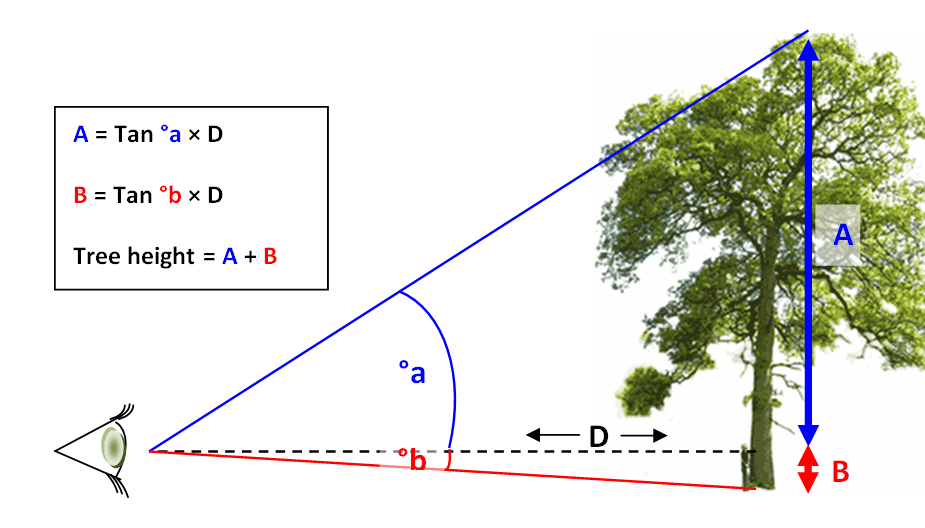
\includegraphics[width=0.8\textwidth]{Images/TreeHeight.png}
	\caption[Measuring Tree Height]{Measuring Tree Height}
	\label{fig:Height}
\end{figure} 
\newpage
These ways of calculating height are time consuming and costly, however, measuring Diameter
at Breast Height (DBH) is a much easier method as it only involves measuring the stem/tree diameter at 1.3m above ground level. We know there is a relationship between DBH and height \cite{10.1093/treephys/tps127}, and this relationship has been used for years to create models by tree species to estimate tree height such as the most commonly used model, the Naslund model:\\ $h(d)=bh + \frac{d^2}{(a+bd)^2}$ \cite{naslund1936skogsforsoksanstaltens}.\\ Where bh is breast height i.e 1.3m, d = DBH ,and a and b are parameters to be defined\\
These formulas have helped improve the accuracy of forestry inventories but are still not as accurate as they could be. Many other variables effect a trees height that aren’t accounted for in models \cite{doi:10.1080/21580103.2014.957354}, such as plot level variables like soil,density of trees per plot and others we cannot yet account for. While the Naslund model takes this into account with the use of two parameters, which can either be fixed or random or both (mixed effect), it’s not enough to get accurate models per species. Fixed effect models are models where we assume that all studies in an analysis has the same \href{https://www.leeds.ac.uk/educol/documents/00002182.htm}{effect size}, ( the quantitative difference between variables) and the difference in the observed versus the estimated is due to sampling error, i.e the model coefficients are fixed.Random is the opposite of this where we assume the effect size varies by study, while mixed effect is a combination of the two.\cite{borenstein2010basic} To improve the models and compare each type to see which is best, to accurately predict the height of a tree, we must analyze forestry data and input species and plot-based models to predict Tree height. This will be done by taking into account all variables that may effect the models. Using R, and packages such as \href{https://cran.r-project.org/web/packages/lmfor/lmfor.pdf}{lmfor} and \href{https://cran.r-project.org/web/packages/tidyverse/tidyverse.pdf}{tidyverse} which are functions for forests bio metrics and a group of packages to analyze data respectively. Models for tree height can be investigated with statistical methods.\newpage
\section{Forestry Terms.}
As we've seen already DBH is diameter of a tree at 1.3m above ground level and tree height is the height of the tree, but to have a clear understanding of the data and create accurate models we need to know more about forestry terms,data and other models
Such important  \href{http://forestlearning.edu.au/about/forest-terminology-explained.html}{Forestry terms} can be found at this link.Some of the more important terms can be found below:
\begin{itemize}
    \item Stem - which is the main body of the tree.
     \item Canopy(similar to crown) - the top level trees consisting of branches and leaves.
     \item log - cut down trees for timber. logging is the production of logs.
     \item stand - a cluster of trees 
     \item Quadratic mean diameter \cite{10.1093/forestscience/13.4.36} -is the average arithmetic mean squared diameters. 
     $\sqrt{\Sigma\frac{DBH^2}{n}} $
     \item \href{https://www.sciencedirect.com/topics/medicine-and-dentistry/forest-plot}{forest plot} is a collective of studies and a visualization of the common effects that the collected studies suggest and their heterogeneity.
     \item Basal area is an important measurement that is used to calculate Stand density,growth of trees and log volume. DBH can be used to calculate Basal area \cite{elledge2010basal} as it is the cross sectional area at breast height of a tree. this can then be used to give a description of the size of the plot i.e basal area of 80 square feet per acre.
\end{itemize}

\section{The Data}
 The Data received was compiled of 13 variables and consisted of 4652 entries.the variables consisted of Qualitative and Quantitative data, as shown below from the first 10 entries of the Data.
The majority of the Heights were not measured as this is what we wish the model to estimate. 3848 missing heights with 803 heights given.\\
A graph is shown below (Figure \ref{fig:Height}) that gives a example of the relationship between height and DBH, as we can see there is an increase in height as the diameter at breast height increases.We see that DBH effects smaller trees more drastically, as DBH increases the scatter-plot is tending to level off. The various sizes of height per DBH however shows there is more variables that effect the height of the tree.
Models used to calculate height estimates for trees are part of the $lmfor$ package in R.

\section{DBH - Height Models}

Height estimation models consisted of mixed effect models that can also be used as fixed effect models or random effect models. \\
The models that are represented below are a few of the models  that have been reviewed and can be found on the \href{https://cran.r-project.org/web/packages/lmfor/lmfor.pdf}{lmfor page.}.
\begin{itemize}
    \item Wykoff is a stand prognosis model from 1982 \cite{wykoff1982user}
    \item Curtis is a model created in 1967s as a Height-diameter and height-diameter age equations for
second-growth Douglas fir\cite{10.1093/forestscience/13.4.365}
\item Meyer is a model created in the 1940s as a mathematical expression for height curves. \cite{meyer1940mathematical}
\end{itemize}
These models are nonlinear curves between Height and DBH. As stated the aim is to examine these models to find an optimal model for each species and from there improve the models by adding more parameters to the model fixed or random depending on which is more adequate. 
\begin{table}[ht]
\centering
\caption{Forestry Data received from Coillte}
\resizebox{\textwidth}{!}{\begin{tabular}{rllrrrrlllrllrr}
  \hline
 & PopulationName & StratumName & PlotId & TreeNumber & DBH & Height & HeightStatus & IsDead & OutsidePlot & MirageCount & LastMeasured & SPP & Windblown & Res.Trees \\ 
  \hline
1 & CE05-H0023 & 42392A-7 &   1 &   1 & 1.25 &  & MISSING & Live & False &   1 & 2017-12-05 12:07:51 & LPS & NA & NA \\ 
  2 & CE05-H0023 & 42392A-7 &   1 &   2 & 1.12 &  & MISSING & Live & False &   1 & 2017-12-05 12:08:23 & LPS & NA & NA \\ 
  3 & CE05-H0023 & 42392A-7 &   1 &   3 & 0.80 &  & MISSING & Live & False &   1 & 2017-12-05 12:08:44 & LPS & NA & NA \\ 
  4 & CE05-H0023 & 42392A-7 &   1 &   4 & 1.10 &  & MISSING & Live & False &   1 & 2017-12-05 12:09:01 & LPS & NA & NA \\ 
  5 & CE05-H0023 & 42392A-7 &   1 &   5 & 0.77 &  & MISSING & Live & False &   1 & 2017-12-05 12:09:25 & LPS & NA & NA \\ 
  6 & CE05-H0023 & 42392A-7 &   1 &   6 & 1.50 &  & MISSING & Live & False &   1 & 2017-12-05 12:09:45 & LPS & NA & NA \\ 
  7 & CE05-H0023 & 42392A-7 &   1 &   7 & 1.01 &  & MISSING & Live & False &   1 & 2017-12-05 12:10:10 & LPS & NA & NA \\ 
  8 & CE05-H0023 & 42392A-7 &   1 &   8 & 1.65 &  & MISSING & Live & False &   1 & 2017-12-05 12:10:25 & LPS & NA & NA  \\ 
  9 & CE05-H0023 & 42392A-7 &   1 &   9 & 1.66 &  & MISSING & Live & False &   1 & 2017-12-05 12:10:46 & LPS & NA & NA \\ 
  10 & CE05-H0023 & 42392A-7 &   1 &  10 & 1.01 &  & MISSING & Live & False &   1 & 2017-12-05 12:11:02 & LPS & NA & NA  \\ 
   \hline
\end{tabular}}
\end{table}

   \begin{tabu}  spread \linewidth {|c|c|c|c|}\hline
        \rowfont{\bfseries}
          Model & Formula & R code  \\ \hline
     Naslund & $\displaystyle h(d)=bh + \frac{d^2}{(a+bd)^2}$ & $ HDnaslund(d, a, b, bh=1.3)$ \\ \hline
     Naslund_2 & $\displaystyle h(d)=bh +  \frac{d^2}{(a+e^{b}d)^2}$ & $HDnaslund2(d, a, b, bh=1.3)$  \\ \hline
     Naslund_3 & $\displaystyle h(d) = bh +  \frac{d^2}{(e^{a}+bd)^2}$ & $HDnaslund3(d, a, b, bh=1.3)$ \\ \hline
     Naslund_4 & $\displaystyle h(d) = bh +  \frac{d^2}{(e^{a}+e^{b}d)^2}$ & $HDnaslund4(d, a, b, bh=1.3)$ \\ \hline
     Wykoff & $\displaystyle h(d)=bh +  e^{(a + \frac{b}{d+1})}$ & $ HDwykoff(d, a, b, bh=1.3)$\\ \hline 
     Curtis & $\displaystyle h(d) = bh + a(\frac{d}{1+d})^b $ & $HDcurtis(d,a,b,bh=1.3)$\\ \hline
     Meyer & $\displaystyle h(d) = bh + a(1-e^{-bd})$ & $HDmeyer(d,a,b,bh=1.3)$\\ \hline 
      \label{tabu:Models}
   \end{tabu} 


\begin{figure}[thb]
	\centering
		\caption[Height_DBH]{Height and Diameter at breast height scatter plot}
	\label{fig:Height}
	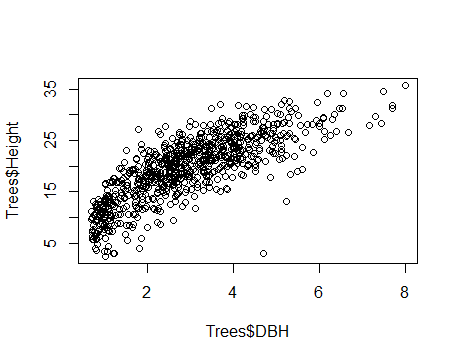
\includegraphics[width=0.5\textwidth]{Images/Height_DBH.png}
	
\end{figure}

\section{Lidar}
Initially research in \href{https://oceanservice.noaa.gov/facts/lidar.html}{LIDAR} and the \href{https://oceanservice.noaa.gov/facts/lidar.html}{models} that are created from the data, was recommended by Coillte associates.LIDAR Stands for Light Detection and Ranging. It works using light, sending pulses of an laser from a plane/helicopter to the ground  measuring how long it takes for the light to return back to the sensor.Using GPS to mark where each pulse of light was emitted it can provide models by geographical position.
This provides accurate terrain models and gives you an inventory through sensing three dimensional forest vegetation.
There are three models that can be created from LIDAR data.
\begin{itemize}
    \item \textbf{Digital Elevation Model (DEM):}A digital elevation model is a 3-D model of the terrain.When you filter out the non ground hits from the pulses light pulses detected by the sensor, you are left with a model of the terrain. this is extremely useful for hydrologic modeling to map the flow of rivers and find watersheds. 
    \item \textbf{Digital Surface Model (DSM):} Digital surface models are taking first returns of the light pulses.it creates a model of the surface including the tree canopy's, buildings and other structures elevated from the surface of the earth.
    \item \href{https://rapidlasso.com/2014/11/04/rasterizing-perfect-canopy-height-models-from-lidar/}{Canopy Height Model:}Canopy height model is the difference between the DSM and the DEM.This can be done by computing DSM and DEM and subtracting the two rasters.\href{http://desktop.arcgis.com/en/arcmap/10.3/manage-data/raster-and-images/what-is-raster-data.htm}{Raster data} is a matrix of pixels in rows and columns. This represents the height of the trees.
\end{itemize}

\begin{figure}[hb]
  \centering
  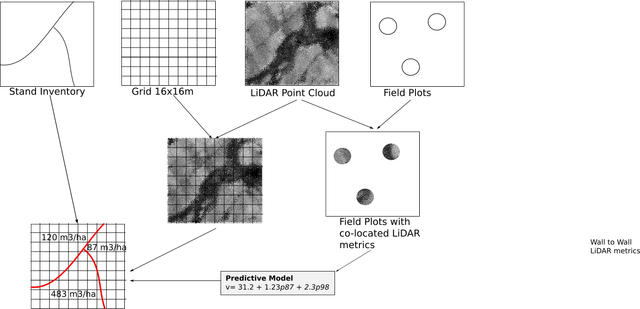
\includegraphics[width=1\linewidth]{Images/LIDAR.png}
  \caption{LIDAR Process}
  \label{fig:DBH_Species}
  \end{figure}
  
\begin{figure}[t]
    \centering
 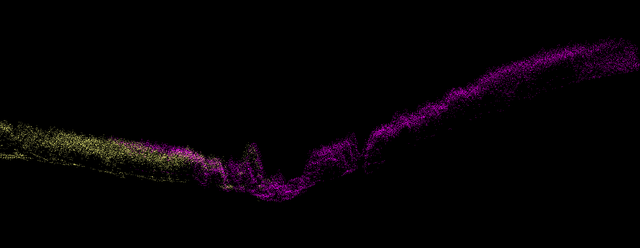
\includegraphics[width=.5\linewidth]{Images/LIDAR_CLOUD.png}
  \caption{Lidar Cloud image}
  \label{fig:LIDAR_CLOUD}
\end{figure}

\begin{figure}[ht]
\centering
\begin{subfigure}{.5\textwidth}
  \centering
 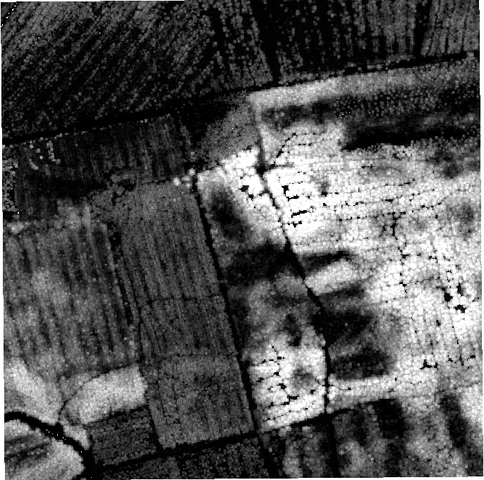
\includegraphics[width=1\linewidth]{Images/CHM.png}
  \caption{Lidar image}
  \label{fig:LIDAR_CLOUD}
\end{subfigure}
\begin{subfigure}{.5\textwidth}
  \centering
 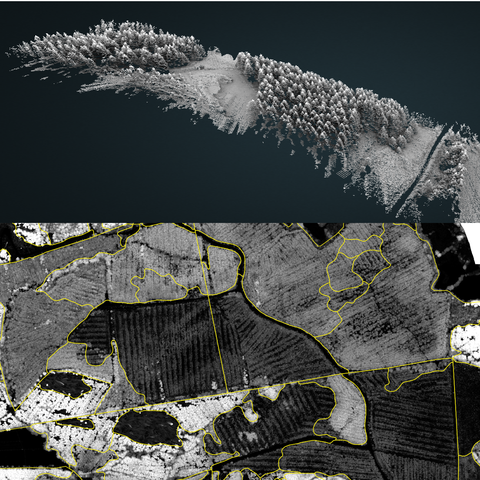
\includegraphics[width=1\linewidth]{Images/3D_pointCloud.png}
  \caption{Above: Canopy Height Model(CHM) - 1-m resolution(black = ground , White are the tallest tree's).
  Below: Segmented canopy height model.}
  \label{fig:LIDAR_CLOUD}
\end{subfigure}
\end{figure}

\chapter{Previous literature}
To learn about forestry industry \href{http://wiki.awf.forst.uni-goettingen.de/wiki/index.php/Category:Forest_inventory}{forestry wiki page} and \href{http://forestlearning.edu.au/about/forest-terminology-explained.html}{Forest Learning} were primarily used to retrieve basic information and have an underlining knowledge of previous literature\\
Previous literature in forestry data spans decades. with Naslunds\cite{naslund1936skogsforsoksanstaltens} and Meyer papers\cite{meyer1940mathematical}  being created in 1936 and 1940 respectively.These models, despite being around for a while, are still relevant today and still being used in literature released in recent years. 
In Lauri Mehtätalo, Sergio de-Miguel, and Timothy G. Gregoire's Modeling height-diameter curves for prediction they examined multiple models \cite{mehtatalo2015modeling}, and interpreted multiple models for different species of trees. First, they tested if each model would converge. If a model didn’t converge it was a sign that the model didn’t fit the data. This was when data was put into the model and the result was not within a certain neighborhood of the estimate, which is explained well in \href{https://www.rasch.org/rmt/rmt11b.htm}{rasch website}.
Once models converge, statistical methods were used such as AIC and BIC to see which models fit best. This was similiar to Ram P. Sharma and Johannes Breidenbach route, illustrated in their paper \cite{doi:10.1080/21580103.2014.957354}.where they use the ordinary least squares (OLS) method, Fit statistics and residual variations to identify a model to use as their base model.They found $Naslund Model$ to be of best fit for their data with one fixed parameter $b=3$. To find variables that would fit the model they had a interesting method of finding the variables to apply to the function. Firstly they found estimates of the parameters of the model. Then fixing these estimates they plotted each stand variable they wished to look at against the parameter estimates,and looked at the variables that had a significant relationship with the parameters. Different combinations of the variables were used and their transforms like square root of a variable were used to improve model fit. \\
Such variables were plot level variables like dominant tree height(hdom) and dominant DBH (ddom), These are the average of the highest 100 values of each.The quadratic mean diameter(qmd) was another variable, N the number of trees per plot and DBH range.\\ 
These 5 variables and more were looked at to see if they had a relationship with the parameters, this was proceeded by getting estimates of the Naslund model which were then plotted against each variable. The five stated above however were the ones that showed a significant relationship.
Adding these to the model as parameters they extended the base model of Naslunds.
Their results found a reduction of AIC and BIC when using two of the plot level variables dominant height and dominant DBH. they found if they included residual heteroskedasticity they got a further reduction of AIC.
This may be due to the fact that ordinary least squares method assumes that variance among the population is constant.\\
A interesting note is that dominant height and dominant DBH were the only two plot level variables the report stated that were independent of thinning.In contrast, the other plot level variables were all affected by thinning which caused complications in the report.The report also stated that mixed effect models gave more accurate results as they took variation by plot into account.\\
While this report took into account prediction variables and took out noise adequately, There was improvements that could be made. This lead to the thinking of other statistical methods that weren't the norm in forestry analysis that could be used. Therefore, a report on the use of the Bayesian Method for tree height - DBH model \cite{zhang2014estimating}.
This report took a interesting way of looking at the models.They describe how the Bayesian method may improve the model as it took the parameters to be random variables. They found that when using the classical maximum likelihood and ordinary least squares method against the Bayesian method, whilst looking at 6 height - diameter models, That the Bayesian method led to narrower confidence intervals for predicted height and parameter estimates had lower confidence intervals also.\\
They used 6 non linear models that were different to the models used in other reports, they found that the Weilbull model gave best fit of data.\begin{equation}
Weibull-  h(d) = 1.3 + a(1-{-b*DBH^c})
\end{equation}
Where $a,b,c$ are three parameters.
Bayes rule as stated in the report at section~3.2\cite{zhang2014estimating},
states that for a vector of data $y= (y_1,y_2,....)$.
And let $\theta$ be a vector of parameters such that $\theta = (\theta_1,\theta_2,....)$ to be estimated. Then Bayes rule can be expressed as:\begin{equation}
\label{eq:Bayes rule}
P(\textbf{y}|\theta) = P(\textbf{y} |\theta)P(\theta ),
\end{equation}
They noted that they are after the conditional distribution of $\theta$ given data $y(p(\theta|y))$. Another method that may be of use that they discussed is the distribution of parameters.stating that many researchers use uninformative normal priors. Alternatively using previous studies, they could construct a prior distribution.
Literature reviewed on the relationship between tree height and DBH have similar results, that mixed models were the most efficient. Heteroscedasticity and plot level variation must be accounted for, and we aim to minimize the prediction intervals.

\chapter{Preliminary Results} 

Looking at the data we see there are 13 variables with 6 qualitative variables and 5 quantitative variables.
The relationship with DBH and Height shown in Fig \ref{fig:Height}, we saw there was a clear relationship between the variables however certain parameters affect the relationship that give it its' variation of heights in the plot.
Looking at the relationship between each variable was next. Knowing that the species and DBH will have an impact on the model, this was looked at in a box-plot to find which species had the highest DBH along with height. With these models we see that there is a large amount of variation per species unexplained.\\
A linear model to identify obscure entries was made, QQ plots showed that entries like 3806 were severe outliers and that there were more changes to be made to improve the model.
Looking at these entries it was found that the tree height status was broken, this brought to question how broken trees will affect the model. This resulted in forward and backward step elimination with BIC values. Using this we found that \\ 

\begin{equation}
      Height \sim DBH + StratumName + SPP + HeightStatus + PlotId
    \end{equation}
    
These, along with ‘Population Name’ will now be looked at to see if its’ presence will improve the models to be used. While population name didn’t come up, it is an important variable and will be used in the future to split up the data to look at each geographical area separately.  \\
For analyzing models, fit statistics per model needs to be gathered to see which model would suit each species. As each species would have different variations in their data, one model won’t suit all.
Therefore, Root Square Mean Error(RSME), Mean absolute error, Chi square test, AIC and BIC will be used to find a base model per species.
Looking at the models by species is an important step. As shown in Figure \ref{fig:SpeciesRelationship}, large amounts of variation in height and DBH relationship is due to species. From researching previous literature on the relationship between DBH and Tree Height, the Naslund model was primarily used.\\
Starting with Naslund, Models were made per species varying in fixed effect, mixed effect and random effect.\\
There are 10 species in the data however there are species that have 4 or less entries. this wont give a accurate estimate of height as there needs to be more data to have a worthwhile model. So, these species will be left to the side for now as models cannot be used for these. Disregarding LPI, GF, and SP models were created for the rest. 
\par
\texttt{$ImputeHeights(DBH, Height, Plot, modelName = "naslund"
, nranp = 1, varf = TRUE,\\ addResidual = TRUE, makeplot = TRUE, level = 1,
 start = NA, bh = 1.3,\\ control = list(),random = NA)$}
 \par
 From the description of the code on \href{https://cran.r-project.org/web/packages/lmfor/lmfor.pdf}{CRAN LMFOR page 12} it can be seen that\\
 DBH - is diameter at breast height variable
 Height - Tree height variable
 Plot - plot id of numeric values usually a plot indices.
 ModelName - specify which model will be used i.e "naslund", "wykoff",etc
 nranp - this tells R if it is mixed, fixed or random model. if nranp = 0 then its a fixed effects model.
 if it is 1 than the first coefficient varies among plots and the others are fixed,
 if it's 2 then 2 coefficients vary among plots,
 and if it's an 3 parameter model than 3 can be picked to vary all parameters among plot.\\
 Initially each version of Naslund models was used per species and used fit statistics to see which is best fit for each model. Each model that was best fit per species would be the base model for that species. Residual plots were also looked at such as Fig 3.1. which is a plot of standardized residuals. This graph shows good fit as standardized residuals should have a normal distribution: $Standardized Residuals \sim \mathcal{N}(0,\,\sigma^{2})\,.$.This plot shows that it has with each vertical line showing $\pm1$ standard deviation from the mean. With each vertical line having close to its centre on 0 it shows the model is of good fit. 
 Once the base model was selected per species, other models were created using other base models in table \ref{tabu:Models} on page \pageref{tabu:Models} such as Wykoff model\cite{wykoff1982user}, curtis model \cite{curtis2000quadratic}, and the meyer model \cite{meyer1940mathematical}.
 % latex table generated in R 3.2.4 by xtable 1.8-3 package
% Fri Nov 02 12:23:07 2018
\begin{table}[ht]
\caption[Species and their models]{Model that best fit the data per species}
\begin{tabular}{rrrr}
  \hline
Species(\href{https://www.forestry.gov.uk/pdf/PF2011_Tree_Species.pdf/$FILE/PF2011_Tree_Species.pdf}{Species code names}) & Entries & R model & Formula\\ 
  \hline
DF (Douglas Fir) & 415 &HDNaslund2() 1 random parameter 
& $h(d)=bh +  \frac{d^2}{(a+e^{b}d)^2}$ \\
  GF (Grand Fir) &   4 & \textcolor{red}{Not enough entries for model}\\ 
  JL (Japanese Larch)& 139 &HDNaslund3() fixed effect model 
  & $h(d) = bh +  \frac{d^2}{(e^{a}+bd)^2}$  \\
  LPI (Lodgepole Pine) &   1 & \textcolor{red}{Not enough entries for model} \\
  LPS (Lodgepole Pine)  & 118 &HDNaslund3() fixed effect model
  & $h(d) = bh +  \frac{d^2}{(e^{a}+bd)^2}$  \\
  NF (Noble Fir)&  58 &HDNaslund2() 1 random parameter 
  &  $h(d)=bh +  \frac{d^2}{(a+e^{b}d)^2}$  \\ 
  NS (Norway Spruce) &  58 &HDNaslund4() 1 random parameter 
  & $h(d) = bh +  \frac{d^2}{(e^{a}+e^{b}d)^2}$\\ 
  SP (Scots Pine) &   2 & \textcolor{red}{Not enough entries for model}\\ 
  SS (Stika Spruce) & 3750 &HDNaslund() 1 random parameter
  &$h(d)=bh + \frac{d^2}{(a+bd)^2}$ \\ 
  WH (Western Hemlock) &  83 &HDNaslund4() 1 random parameter & $h(d) = bh +  \frac{d^2}{(e^{a}+e^{b}d)^2}$  \\ 
   \hline
\end{tabular}
\end{table}

\begin{figure}[h]
    \centering
    \caption[Plot and qqplot]{Example of sample plot, and a QQplot}
    \begin{subfigure}{.5\textwidth}
      \centering
      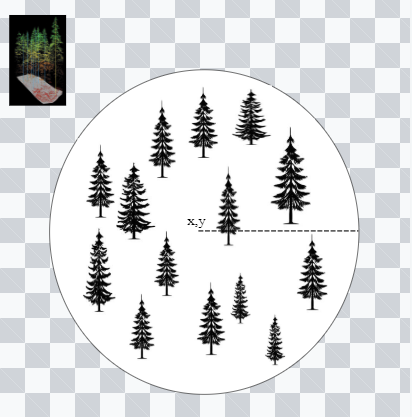
\includegraphics[width=.8\linewidth]{Images/Captureplotsize.PNG}
      \caption{fixed radius circular plots used to collect samples}
      \label{fig:fixed radius circular plots used to collect samples}
    \end{subfigure}
    \begin{subfigure}{.5\textwidth}
     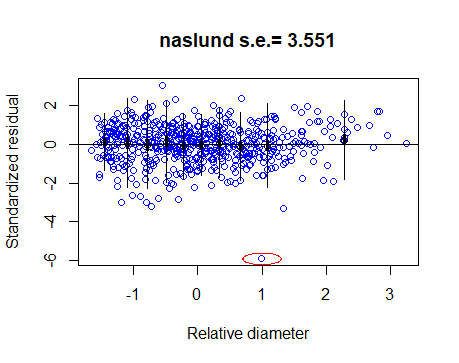
\includegraphics[width=1.2\linewidth]{Images/SS_Residualsplot.png}
    \caption{Residual Plot for Stika Spruce base model.With normal distribution, having only one extreme outlier}
    \label{fig:my_label} 
    \end{subfigure}
    
\end{figure}

\begin{figure}[h]
\centering
\caption[relationship]{DBH - Height plot with boxplots showing species effect on DBH and height}
\begin{subfigure}{.5\linewidth}
\centering
\caption{DBH-Height graph with Naslund model(in red)}
      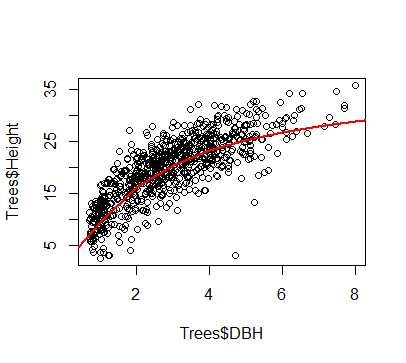
\includegraphics[width=1\linewidth]{Images/Naslund_Fun.png}
\end{subfigure}
\begin{subfigure}{.5\textwidth}
  \centering
  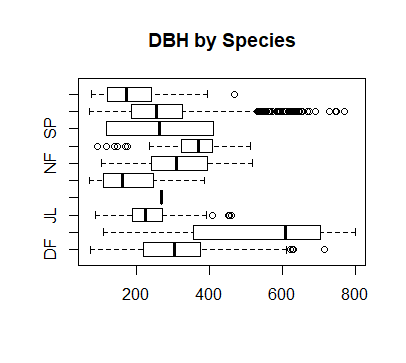
\includegraphics[width=1\linewidth]{Images/DBH_SPECIES.png}
  \caption{DBH by Species}
  \label{fig:DBH_Species}
\end{subfigure}%
\begin{subfigure}{.5\textwidth}
  \centering
 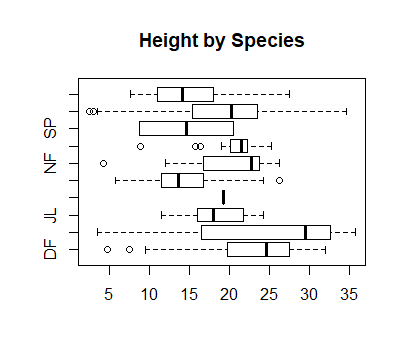
\includegraphics[width=1\linewidth]{Images/HeightBySpecies.png}
  \caption{Height by Species}
  \label{fig:Height_Species}
\end{subfigure}
\label{fig:SpeciesRelationship}
\end{figure}

\begin{figure}[t]
    
\end{figure}




\chapter{Further Research}
To continue research into forestry procedures and to ensure there was a strong understanding on the benefits of creating models to estimate tree height, Coillte provided a \href{https://www.agriculture.gov.ie/media/migration/forestry/nationalforestinventory/nationalforestinventorypublications/4350NFIMethodology.pdf}{Field Procedure and Methodology booklet } by the Department of Agriculture, Food and Marine.\\
The booklet had a surplus of information on forests bio-metrics, how to measure and record said bio-metrics, and how they effect each other. The booklet was very beneficial for interpreting new variables that were not in the previous data sets. This was especially the case with elevation, aspect and slope.The new data set as a whole will be discussed in further detail in the next chapter. From the booklet page 36, it states that Elevation has a negative effect on Tree growth i.e. DBH and height. Altitude brings many factors that affect the growth of trees, sparse forests in high altitude gives to impoverished soils with little decaying matter to keep the soil healthy. The lack of nutritious soils leads to slow growing trees which has its benefits as they last longer but will not grow as well as low altitude forests.\cite{doi:10.1111/j.1365-2745.2007.01280.x}\\
There is a definition called Tree-line. The tree-line is the elevation limit as to which a tree can grow. As altitude increases it becomes harder and harder for trees to grow and reproduce. The tree-line varies by location due to several factors such as temperature, air pressure and soil.\cite{Odland_2015} 
 %   https://homeguides.sfgate.com/effects-land-elevation-tree-growth-31433.html %%
 \begin{figure}[htb]
    \centering
 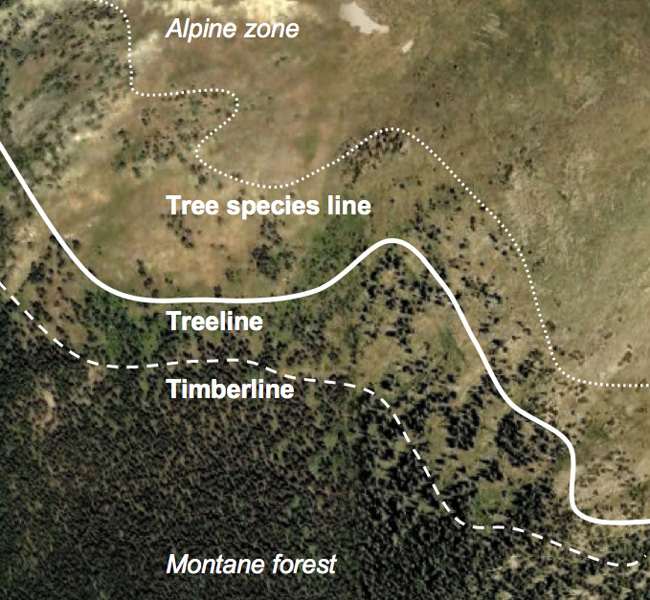
\includegraphics[width=.5\linewidth]{Images/TreeLine.jpg}
  \caption{Image of Tree Line in a montane forest}
  \label{fig:Mangroves}
\end{figure}
%%%%%%%%%%%% Ref %%%%%%%%%% 
\newpage
Aspect is in reference to the orientation of the slope. Aspect can indicate how much the trees are exposed to the natural forces. For example research into north and south facing forests in a semiarid trans-Himalayan valley, found that north facing forests grew faster than south facing forests. \cite{maaren2015facing}
%%%%%%% ref%%%%%
A south western slope would be more open to winds and this affects forests growth by spreading seeds and in turn the forest grows sparsely. Aspect has been in recent times interpreted in angles and cosine and sine to identify the impact it has on the forest. Another study found that forest canopy height was largely affected by aspect when looking at forests in New South Wales.\cite{hu2018evaluating}\\ %%% is this true ? Ref%%%%
Slope is the steepness of a plot and this effects how hard it is to traverse the forest. With a sloped land soil may become more loose and lead to unstable foundation for the trees to grow. \href{https://pdfs.semanticscholar.org/6e74/b49c6c3f6c37ed93575f7f9e48878d30b391.pdf}{Xylem} is a transportation tissue in trees that transports water,minerals and nutrients throughout the tree. Xylem is extremely important for trees overall health and growth. Research into sloped forests have shown that there is a significant difference in xylem structure due to the slope of the terrain.\cite{barij2007does}
%%%%%%%% Ref study %%%%%%%%%%%%%%%


% ask as variance is well different for each variable %

Soil has a big impact on the health of a forest and trees growth. The Soil content describes how much nutrients and moisture trees in a forest receive. In general soil has two broad categories: Peat and Mineral soil. Within these two groups soil varies as it can have a mixture of both categories for example some soil types could be 40\% Peat and 60\% Mineral, however for this research we will be keeping to these two groups. In figure \ref{fig:Mineral vs Peat} we can see how mineral soil has more height on its trees than peat with the same DBH.
%%%%%%% PEAT AND SOIL DESCRIPTIONS %%%%%%%%%%%%%%
% describe the difference between peat and mineral soil
% put up pictures of aspect, slope tree line mineral and peat soil and all of that 
% latex table generated in R 3.5.2 by xtable 1.8-3 package
% Tue Mar 05 11:43:00 2019


%%%%%%%%%% REMOVE THESE TWO TABLES AS THEY DONT MAKE SENSE%%%%%%%%%%%%%%%%%%%


% latex table generated in R 3.5.2 by xtable 1.8-3 package
% Tue Mar 05 11:43:36 2019



\chapter{New Data Set}



% latex table generated in R 3.5.2 by xtable 1.8-3 package
% Wed Feb 27 19:06:32 2019
\begin{table}[ht]
\centering
\scalebox{.48}{
\begin{tabular}{rllrlrrrlllrlrrrrrrrrll}
  \hline
 & id & SPP & DBH\_mm & Height & Forest & County & Compartment & Sub & Method & aspect\_mean & asp\_median & elevation\_mean & elevation\_median & slope\_mean & slope\_median & Coast & Elevation\_Group1 \\ 
  \hline
1 & 00075B1  & MP & 246 & & MO06 & MO & 00075B &   1 & Plots & 246.40 & 273.25 & 65.41 & 66.62 & 6.22 & 6.16 & West & Low \\ 
  2 & 00075B1 & LPS & 209 & & MO06 & MO & 00075B &   1 & Plots & 246.40 & 273.25 & 65.41 & 66.62 & 6.22 & 6.16 & West & Low \\ 
  3 & 00075B1 & LPS & 232 & & MO06 & MO & 00075B &   1 & Plots & 246.40 & 273.25 & 65.41 & 66.62 & 6.22 & 6.16 & West & Low \\ 
  4 & 00075B1  & LPS & 293 & & MO06 & MO & 00075B &   1 & Plots & 246.40 & 273.25 & 65.41 & 66.62 & 6.22 & 6.16 & West & Low \\ 
  5 & 00075B1  & LPS & 266 & & MO06 & MO & 00075B &   1 & Plots & 246.40 & 273.25 & 65.41 & 66.62 & 6.22 & 6.16 & West & Low \\ 
  6 & 00075B1  & LPS & 169 & & MO06 & MO & 00075B &   1 & Plots & 246.40 & 273.25 & 65.41 & 66.62 & 6.22 & 6.16 & West & Low \\ 
  7 & 00075B1 & LPS & 168 & & MO06 & MO & 00075B &   1 & Plots & 246.40 & 273.25 & 65.41 & 66.62 & 6.22 & 6.16 & West & Low \\ 
  8 & 00075B1 & LPS & 247 & 15.60 & MO06 & MO & 00075B &   1 & Plots & 246.40 & 273.25 & 65.41 & 66.62 & 6.22 & 6.16 & West & Low \\ 
  9 & 00075B1 & MP & 272 & & MO06 & MO & 00075B &   1 & Plots & 246.40 & 273.25 & 65.41 & 66.62 & 6.22 & 6.16 & West & Low \\ 
  10 & 00075B1 & MP & 156 & & MO06 & MO & 00075B &   1 & Plots & 246.40 & 273.25 & 65.41 & 66.62 & 6.22 & 6.16 & West & Low \\ 
   \hline
\end{tabular}}
\end{table}
To continue the work Coillte sent on a SQL data base containing about 72000 trees.The Data base consisted of several data-sets. With different data sets containing relevant variables, a new data set containing the necessary variables was to be created.\\
To do this SQLite had to be installed. SQL stands for Structured Query Language. It is used for data base management. Once \href{https://www.sqlite.org/index.html}{SQLite} was downloaded the data base could be managed.\\
It was discovered that three data sets contained all the necessary variables. With this each of the three data sets was exported onto R where using merge() function and paste function the three data sets were joined by two variables, "Sub" and "Compartment".This new Data-set contained 22 variables. Out of these 22 variables there was Forest,plot id,SPP,DBH mm,Height,Compartment,Elevation mean and Median,slope mean and median,aspect mean and median. These were the variables that were of most interest. Other variables like Sub,id.x and id.y were of no use once the three data sets were combined.\\
Once the data set was ready to be used. Each variable was looked into and plotted to see its impact on other variables especially DBH MM and Height.\\
Creating a function that used piping,merge and similiar functions two new variables were added. These were County and Coast. County was found by selecting the first two letters of the forest column and in turn County was used to create Coast variable.\\
for Coast it was chosen to have West, Inland, and South and East Coast combined. This was due to there being less counties with forests in the south and east.\par
The R code for adding an County column to the data set is as below: 
\begin{frame}
\begin{verbatim}
addCounty = function(myData){
  myData <- myData %>% mutate(County=substr(Forest,1,2),
                              Forest=substr(Forest,1,4)) %>%
  dplyr::select(1:Forest,County, everything())
  
  return(myData)
}

\end{verbatim}
\end{frame}
The R code for using County to create Coast column for the data set: 
\begin{frame}
\begin{verbatim}
addCoast = function(myData){
  myData <- myData %>% mutate(Coast = "Inland")
  myData$Coast[myData$County %in% c("DL","LM","MO","SO",
                                  "GY","CE","KY")] ="West"
  myData$Coast[myData$County %in% c("WX","WW","DN","LH",
                                  "MH","CK","WD")] = "SouthEast"
  myData$Coast= factor(myData$Coast,levels =  c("West","Inland","SouthEast"))
  return(myData)
}
  \end{verbatim}
\end{frame}



% latex table generated in R 3.5.2 by xtable 1.8-3 package
% Thu Feb 28 12:36:03 2019
\begin{table}[ht]
\centering
\caption{Table of Elevation by Coast}
\begin{tabular}{rrr}
  \hline
 & Low & High \\ 
  \hline
West & 30375 & 6685 \\ 
  Inland & 10387 & 3946 \\ 
  South \& East & 9048 & 10076 \\ 
   \hline
\end{tabular}
\end{table}

Variables like elevation and County have a clear relationship. Using Anova table below we can see that both County and Elevation Group1
which is two groups:\\
$low = 0 -> 250m and High = 250->600$\\
and their interaction term have a effect on height. \href{https://www.itl.nist.gov/div898/handbook/prc/section4/prc433.htm}{Anova} is a way of hypothesis testing.\\
The Null Hypothesis is that the means per grouping are equal :
$\mu_1 = \mu_2 = .... = \mu_n$. \\
While the Alternative hypothesis is that the means per groups are not equal : $\mu_1 \neq \mu_2 \neq .... \neq \mu_n$.\\
To continue with this discovery a table was plotted of coast and elevation which as seen below shows us that there is some relationship between elevation and geographical location in terms of West coast, South and East coast, and Inland.
Next was to Stratify the data by selecting species, to do this species was split into three categories: Stika Spruce, Broadleaf and other spruces. Now that we had groups of species stika spruce was chosen to do the initial testing. A table was created of elevation group vs species group to see the relationship they had. This was split into 4 tables by Coast. We can see that the majority of Spruces grew in the West regardless, While all high elevation spruces grew in the South and East.
%%%%%%% Fix code and write more about this %%%%%%%%%%%%%%%%%

%%%%%%%% Soil data was received however it had a complex 5 % issue with applying it effectively to the function.  % While it was given late also resulted in it being hard % construct a method of adding it to the function due to it % being different per plot ,not necessarily being the same % soil type in the whole forest.
Soil has a important impact on tree growth, but it was not in any of the data sets given. Contacting Coillte I received a data set that had soil type and had variables such as sub and compartment so it was possible to connect it to the main data set. With soil in two columns: $Non peat percent$ and $Peat percent$. \\
These two columns summed to 100\%.( i.e if  Non peat percent was 30\% then peat percent was 70\%) There was some soils that were 100\% mineral or 100\% peat, however there were few of these and it varied by plot. This meant in a forest you could have several variations of soil to account for.

\begin{figure}[hb]
  \centering
  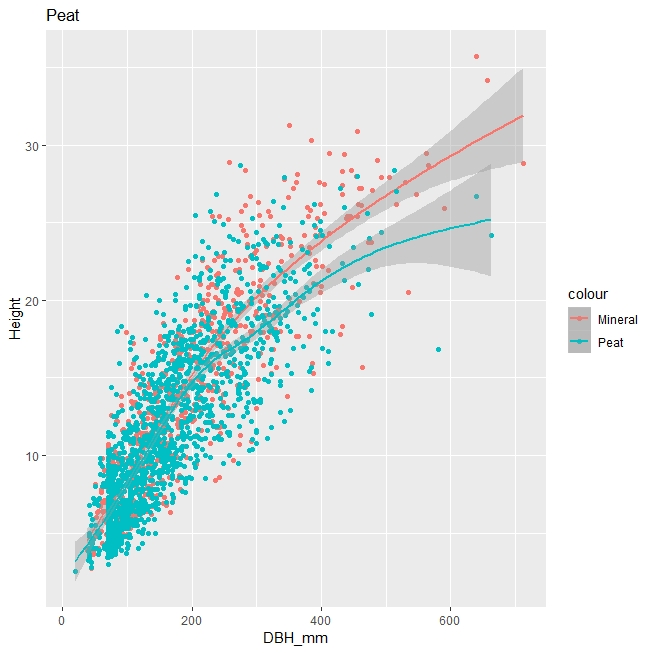
\includegraphics[width=.8\linewidth]{SoilPlot.jpeg}
   \caption{Mineral Vs Peat Plot}
  \label{fig:Mineral vs Peat}
  \end{figure}
  
%To interpret the data efficiently by region a map of Ireland showing information by forest plot was discussed. This would be a outline of the Republic of Ireland with county regions as well. With forests tree height estimations and other forest bio metrics on the map it would increase the ease of visualising the effects of geographical region.\\ 



% latex table generated in R 3.5.2 by xtable 1.8-3 package
% Thu Feb 28 12:02:29 2019
\begin{table}[th]
\centering
\begin{tabular}{lrrrrr}
  \hline
 & Df & Sum Sq & Mean Sq & F value & Pr($>$F) \\ 
  \hline
County & 24 & 9788.33 & 407.85 & 12.93 & 0.0000 \\ 
  Elevation\_Group1 & 1 & 1178.31 & 1178.31 & 37.34 & 0.0000 \\ 
  County:Elevation\_Group1 & 17 & 4629.11 & 272.30 & 8.63 & 0.0000 \\ 
  Residuals & 4783 & 150920.88 & 31.55 &  &  \\ 
   \hline
\end{tabular}
\end{table}


% latex table generated in R 3.5.2 by xtable 1.8-3 package
% Mon Mar 04 13:32:49 2019
\begin{table}[ht]
\centering
\begin{tabular}{lrrrrr}
  \hline
 & Df & Sum Sq & Mean Sq & F value & Pr($>$F) \\ 
  \hline
Coast & 2 & 457877.43 & 228938.71 & 40.38 & 0.0000 \\ 
  Elevation\_Group1 & 1 & 49325.46 & 49325.46 & 8.70 & 0.0032 \\ 
  Coast:Elevation\_Group1 & 2 & 910067.19 & 455033.60 & 80.25 & 0.0000 \\ 
  Residuals & 41715 & 236525845.06 & 5670.04 &  &  \\ 
   \hline
\end{tabular}
\end{table}
\begin{figure}[t]
    \centering
 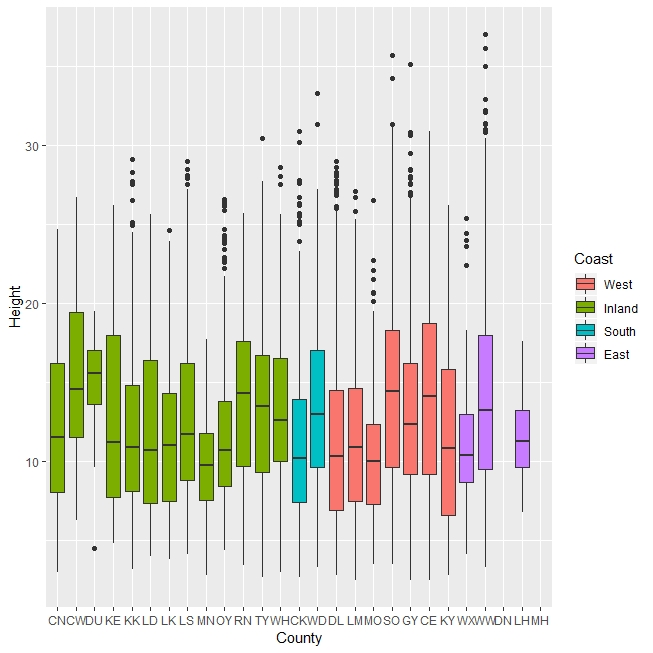
\includegraphics[width=.9\linewidth]{Images/County Height by Coast.jpeg}
  \caption{Box-Plot of Tree Height by County}
  \label{fig:Box-Plot of Tree Height by County}
\end{figure}

\chapter{Results}

Sub setting the data with respect to Species group, Elevation, County and Coast as mentioned above. Each subset was analysed and then used to estimate tree heights in their subsets. Initially Stika Spruce was used to see how sub setting the data impacted the accuracy of the Naslund Function. Creating an extra subset of all Stika Spruce trees and estimating these trees heights to create a base model to compare how much more accurate sub setting the data more would be. Analysing the residual plots we saw a increase in overall accuracy. Some subsets had little improvement for example subset of stika spruce of medium elevation ( 200-400m above sea level) in the West Coast had similar residual plots to a subset of all Stika Spruce with the standard error both being roughly 2.6 . \\

Seeing this improvement in estimating tree height, the Akaike information criterion (AIC), mean absolute error (MAE) and the root mean squared error (RMSE) were calculated to gain a better description on how it effected the accuracy of the function.\\

There was an visible improvement in the functions accuracy, with residual plots showing to be normal the other three species groups were put through the same proccess.
The three remaining species groups were ``Broadleaf", ``Other Spruce" and ``Other". \\

As with the stika spruce models there was a clear improvement in the prediction of tree height. However some subsets did not have enough trees to be able to use the function. 
%%%%%%%%%%% STIKA SPRUCE %%%%%%%%%%%
% latex table generated in R 3.5.2 by xtable 1.8-3 package
% Tue Mar 12 20:11:10 2019
\begin{table}[ht]
\centering
\captionof{table}{Stika Spruce} \label{tab:Stika Spruce} 
\begin{tabular}{rlrrr}
  \hline
 & Region & RMSE & MAE & AIC \\ 
  \hline
1 & SouthEastHigh & 3.07 & 2.45 & 1143.84 \\ 
  2 & SouthEastMedium & 3.05 & 2.33 & 4007.70 \\ 
  3 & SouthEastLow & 2.39 & 1.83 & 1134.08 \\ 
  4 & InlandHigh & 1.32 & 1.01 & 23.58 \\ 
  5 & InlandMedium & 2.75 & 2.17 & 2280.14 \\ 
  6 & InlandLow & 2.58 & 1.99 & 1676.55 \\ 
  7 & WestHigh & 0.00 & 0.00 & 0.00 \\ 
  8 & WestMedium & 2.95 & 2.31 & 4563.77 \\ 
  9 & WestLow & 2.82 & 2.20 & 8384.05 \\ 
  10 & All & 2.90 & 2.24 & 23498.95 \\ 
   \hline
\end{tabular}
\end{table}

%%%%%%%%%%%%%% BROADLEAF %%%%%%%%%%%%%%
% latex table generated in R 3.5.2 by xtable 1.8-3 package
% Tue Mar 12 20:11:44 2019
\begin{table}[ht]
\centering
\captionof{table}{Broad Leaf} \label{tab:Broad Leaf} 
\begin{tabular}{rlrrr}
  \hline
 & Region & RMSE & MAE & AIC \\ 
  \hline
1 & WestHigh & 0.00 & 0.00 & 0.00 \\ 
  2 & WestMedium & 2.08 & 1.64 & 51.39 \\ 
  3 & WestLow & 3.04 & 2.38 & 1915.54 \\ 
  4 & All & 2.97 & 2.27 & 6781.05 \\ 
   \hline
\end{tabular}
\end{table}
%%%%%%%%%%%%%%%%% Other Spruce %%%%%%%%%%%%%%
% latex table generated in R 3.5.2 by xtable 1.8-3 package
% Tue Mar 12 20:12:34 2019
\begin{table}[ht]
\centering
\captionof{table}{Other Spruce} \label{tab:Other Spruce} 
\begin{tabular}{rlrrr}
  \hline
 & Region & RMSE & MAE & AIC \\ 
  \hline
1 & SouthEastHigh & 0.00 & 0.00 & 0.00 \\ 
  2 & SouthEastMedium & 2.61 & 1.99 & 1533.15 \\ 
  3 & SouthEastLow & 2.94 & 2.22 & 1530.57 \\ 
  4 & InlandHigh & 1.92 & 1.43 & 110.29 \\ 
  5 & InlandMedium & 2.38 & 1.77 & 653.52 \\ 
  6 & InlandLow & 2.56 & 1.92 & 936.83 \\ 
  7 & WestHigh & 0.00 & 0.00 & 0.00 \\ 
  8 & WestMedium & 2.68 & 2.22 & 206.90 \\ 
  9 & WestLow & 2.66 & 1.95 & 700.75 \\ 
  10 & All & 2.87 & 2.16 & 5698.39 \\ 
   \hline
\end{tabular}
\end{table}
%%%%%%%%%%%%%%%%% Other %%%%%%%%%%%%%%
% latex table generated in R 3.5.2 by xtable 1.8-3 package
% Tue Mar 12 20:13:23 2019
\begin{table}[ht]
\centering
\captionof{table}{Other species} \label{tab:Other species} 
\begin{tabular}{rlrrr}
  \hline
 & Region & RMSE & MAE & AIC \\ 
  \hline
1 & SouthEastHigh & 0.00 & 0.00 & 0.00 \\ 
  2 & SouthEastMedium & 3.06 & 2.33 & 951.31 \\ 
  3 & SouthEastLow & 3.13 & 2.30 & 962.01 \\ 
  4 & InlandHigh & 2.23 & 1.66 & 94.28 \\ 
  5 & InlandMedium & 2.79 & 2.27 & 735.37 \\ 
  6 & InlandLow & 2.60 & 2.04 & 2361.61 \\ 
  7 & WestHigh & 0.00 & 0.00 & 0.00 \\ 
  8 & WestMedium & 2.22 & 1.74 & 2593.09 \\ 
  9 & WestLow & 2.73 & 2.06 & 5527.09 \\ 
  10 & All & 2.73 & 2.06 & 5527.09 \\ 
   \hline
\end{tabular}
\end{table}
%then I looked at splitting by elevation in 2 splits to 3 %maybe 4 and 5 next,
%Then Coast and county to see how this effected the dataset,
%%looking at mae and rmse to see if there is a improvement
%the improvement was interpreted as because of this and that.
%I combined all datasets and added all variables by a function to increase time proficiency.
%looked at accuracy in respects to altitude and geographical location and peat and mineral to see which had the most unexplained variations.

%with this i saw a decreSE IN ACCURACY OF model in some respects but a overall increase in accuracy

%what next did i do, i split variables and put through the function and looked at how they fit the data. had discussions about it. i compiled 



\chapter{Conclusion}
Tree height is an complicated tree bio metric that is influenced by many factors. From research and analysis of Data, it was found that there is a lot of noise that needs to be reduced. Estimating tree height has many factors that are complicated to apply to models for estimating height. Using the variables given we can get a rough estimate of height. Looking at figure \ref{fig:Height} there's visible Heteroscedasticity that effects a models accuracy. Stratifying the data with respect to variables had some beneficial effects but it varied by elevation and coast subsets. Such as for Stika Spruce \ref{tab:Stika Spruce} for forests in the South and East at elevation above 400 metres there was a increase in the root mean squared error from 2.9 to 3.07 and mean absolute error from 2.24 to 2.45. However forests that were in the Inlands and elevation above 400 metres decreased in both, with root mean squared error decreasing from 2.9 to 1.32 and mean absolute error decreasing from 2.24 to 1.01. However all AIC's decreased dramatically showing a big improvement in the models fit.\\
The overall lack of improvement in these regions shows it could be that sub-setting the data in this way has little benefit.   

there was a visible decrease in the functions residuals as factors were accounted for. 
Using AIC (used for seeing how well a model fits the data) we saw the model improve drastically to fit the data.

\par

The analysis of the forest inventory data was an initial step into creating accurate \href{https://www.fs.fed.us/nrs/pubs/gtr/gtr-nrs-p-167papers/27-larsen_2016-CHFC.pdf}{taper equations}. Taper equations are used to find an estimate of the diameter of the tree at any given height.\\
This will give you the volume of wood you have per forest which is crucial for keeping accurate inventory of forests. 



\chapter{R course, Pete Bunding and Osian Roberts Presentation.}


Continuing the analysis of the data, it was visible that there was a lack of R coding skills that were slowing the projects progress. To solve this situation, an Cork \href{https://www.meetup.com/Cork-Ireland-R-Users-Group/}{R user group workshop} by Joe Blogss was attended to improve R coding and interpretation of the data and results.\\
This workshop focused on the Tidyverse package that is in R. Tidyverse is used to maintain a clean data set and code, while teaching you how to visually represent data and interpret data as efficiently as possible. The workshop fine tuned the basic essential R skills that helped bring out more benefits in using R.\\
It was taught using examples that the lecturer worked on himself. These examples were of medical treatments and new drug trials. They were of great use to have hands on work using these new codes, and to understand how it works and why we should implement it into our work. The new skills learnt were instantly used in analysing the forestry data, creating neat code interpretable code, keeping data sets orderly and more descriptive plots.\\

 \href{https://www.eorc.jaxa.jp/ALOS/kyoto/jan2017_kc23/pdf/1-09_KC23_GMW-Bunting.pdf}{Pete Bunding} and his PHD student \href{https://pure.aber.ac.uk/portal/en/persons/osian-dafydd-roberts(a3ce4766-2a73-4338-9993-f5ab467767ec).html}{Osian Roberts} from Aberystwyth University, who are currently working on \href{https://www.globalmangrovewatch.org/author/gmwpjb/}{The Global Mangrove Watch: monitoring of mangrove forests globally} which can be viewed in the link. and Forest bio metrics with airborne LiDAR, machine learning and Monte Carlo ray tracing simulations respectively, were presenting there research in University of Limerick during January. With their research being of great interest to Coillte, it was suggested to watch the presentation. Their presentations were an interesting view on the use of mathematical models, statistics and coding to supervise and maintain important natural resources. \\
Osian Roberts PHD is on the aim to decrease prediction error from 20\% in predicting forests attributes using machine learning and Monte Carlo ray tracing simulations. \\
The presentation lasted roughly an hour and a half to two hours and had Pete and Osian discuss their research up to then in detail. Describing programs used, how they started the projects, calculations, improvements, problems that arose and their results so far.\\
Osian's research was started due to retrieving forest biometrics requires a large Forest inventory which is expensive and time consuming. Instead foresters use regression models from samples of forest plots.This is where foresters take a sample of trees from a forest and measure all the biometrics of these trees and use this to interpret the forest instead of measuring every tree, then using regression models to see the relationship each forest biometric had with each other.\\ This has a prediction error of 20\%. With the use of machine learning and simulators he was able to run multiple simulations to test his hypothesis. The results have being promising so far, showing that a Monte Carlo ray tracing simulator can produce reliable data that describes the forest as a whole from sample sets with a lower prediction interval.

%%%%%%%%% Reference%%%%%%%%%%%%%%%%%%

Pete Bunding's research consisted of the creation of the first global monitoring system for mangroves forests. Using an machine learning approach based on random forest algorithm and a new map to image system, Pete was able to create a monitoring system that is $95.25\%$ accurate, $2.5\%$ omission and a $6\%$ commission.\\
Pete found that there is a annual $-0.29\%$ decrease in mangrove forests globally. However places like Indonesia have seen $20\%$ decrease in their mangrove forests from 1996 to 2016. Monitoring the mangroves is of great environmental benefit. Being easy to access data on the loss and gains of these forest is important to maintain the flora and fauna that flourish in these regions.   
\begin{figure}[bth]
    \centering
 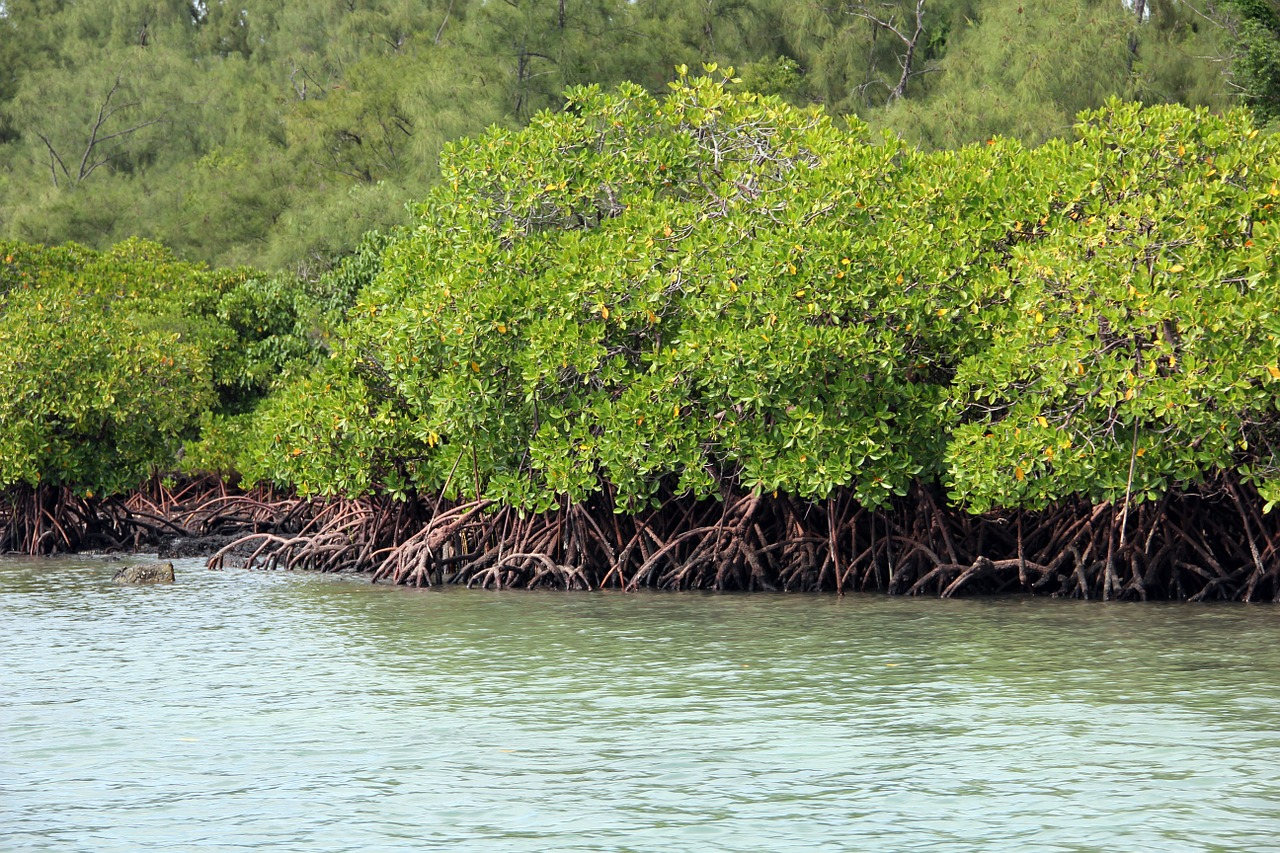
\includegraphics[width=.5\linewidth]{Images/Mangroves.jpg}
  \caption{Mangroves in Indonesia}
  \label{fig:Mangroves}
\end{figure}
%%%%%%%%%%%% reference this  %%%%%%%%%%%%%%%%%%%%%
\bibliography{FYP.bib}
\bibliographystyle{plain}
\end{document}

